
\begin{definition}[\textbf{Cuadrilátero}]
Un \textit{cuadrilátero} es la unión de cuatro segmentos coplanares que se intersecan solo en sus extremos y que son determinados por cuatro puntos de los cuales tres de ellos son no colineales.
\end{definition}

\begin{definition}[\textbf{Cuadrilátero convexo}]
    Un cuadrilátero es \textit{convexo} si, dados dos puntos cualesquiera $\pt{A}$ y $\pt{B}$ en su interior, todos los puntos del segmento $\seg{AB}$ están en el interior de éste.
\end{definition}

\begin{definition}[\textbf{Cuadrilátero no convexo}]
    Un cuadrilátero es \textit{no convexo} (cóncavo), si dados dos puntos $\pt{A}$ y $\pt{B}$ en su interior, algunos de los puntos del segmento $\seg{AB}$ están en el exterior de éste.
\end{definition}

\begin{definition}[\textbf{Ángulos opuestos}]
    Dos ángulos son opuestos si no tiene en común un lado del cuadrilátero.
\end{definition}

\begin{definition}[\textbf{Lados consecutivos}]
    Dos lados son consecutivos si tienen un extremo en común.
\end{definition}

\begin{definition}[\textbf{Ángulos consecutivos}]
    Dos ángulos son consecutivos si tienen un lado en común del cuadrilátero.
\end{definition}

\begin{definition}[\textbf{Diagonal de un cuadrilátero}]
    Una diagonal de un cuadrilátero es un segmento determinado por dos vértices no consecutivos.
\end{definition}

\begin{theorem}
    Las diagonales de un cuadrilátero convexo siempre se intersecan.

    \begin{figure}[!h]
        \centering
        \begin{tikzpicture}[rotate=90]
    \tkzDefPoint(0,0){A} % Define el primer punto
    \tkzDefPoint(2,1){B} % Define el segundo punto
    \tkzDefPoint(3,3){C} % Define el tercer punto
    \tkzDefPoint(1,4){D} % Define el cuarto punto

    \tkzDrawPolygon(A,B,C,D) % Dibuja el cuadrilátero
     % Dibuja las diagonales
    \tkzDrawSegments(A,C B,D)

    % Encuentra el punto de intersección de las diagonales
    \tkzInterLL(A,C)(B,D) \tkzGetPoint{E}
    \tkzDrawPoint(E)
       
    % Etiqueta los puntos
    \tkzLabelPoints[below](A,D,E)
    \tkzLabelPoints[above](C,B)

\end{tikzpicture}
        \caption{Cuadrilátero convexo}
        \label{fig:theorem9}
    \end{figure}

\end{theorem}

\begin{theorem}
    En un cuadrilátero, la suma de los ángulos internos es igual a $\degs{360}$.
\end{theorem}

\clearpage

\subsection{Paralelogramos}

    \begin{definition}[\textbf{Distancia entre dos rectas paralelas}]
    La distancia entre dos rectas paralelas es la distancia de un punto de una recta a la otra recta.
\end{definition}

\begin{theorem}
    En un paralelogramo dos lados opuestos cualesquiera son congruentes.
\end{theorem}

\begin{theorem}
    En un paralelogramo dos ángulos opuestos cualesquiera son congruentes.
\end{theorem}

\begin{figure}[!h]
    \centering
    \begin{tikzpicture}
    \tkzDefPoint(0,0){A} % Define el primer punto
    \tkzDefPoint(4,0){B} % Define el segundo punto
    \tkzDefPoint(6,2){C} % Define el tercer punto
    \tkzDefPoint(2,2){D} % Define el cuarto punto

    \tkzDrawPolygon(A,B,C,D) % Dibuja el paralelogramo

    % Dibuja los ángulos marcados
    \tkzMarkAngle[arc=l,size=0.5cm](B,A,D)
    \tkzMarkAngle[arc=l,size=0.5cm](D,C,B)
    
    \tkzMarkAngle[size=0.3cm](A,D,C)
    \tkzMarkAngle[size=0.4cm](A,D,C)
    
    \tkzMarkAngle[size=0.3cm](C,B,A)
    \tkzMarkAngle[size=0.4cm](C,B,A)

    % Marca los lados congruentes
    \tkzMarkSegment[mark=||](A,B)
    \tkzMarkSegment[mark=||](C,D)
    \tkzMarkSegment[mark=|](A,D)
    \tkzMarkSegment[mark=|](B,C)

    % Etiqueta los puntos
    \tkzLabelPoints[below](A,B)
    \tkzLabelPoints[above](C,D)
\end{tikzpicture}
    \caption{Ángulos opuestos congruentes}
    \label{fig:theorem10}
\end{figure}

\begin{theorem}
    En un paralelogramo dos ángulos consecutivos cualesquiera son suplementarios.

    \begin{figure}[!h]
        \centering
        \begin{tikzpicture}
    \tkzDefPoint(0,0){A} % Define el primer punto
    \tkzDefPoint(4,0){B} % Define el segundo punto
    \tkzDefPoint(6,2){C} % Define el tercer punto
    \tkzDefPoint(2,2){D} % Define el cuarto punto

    \tkzDrawPolygon(A,B,C,D) % Dibuja el paralelogramo

    % Dibuja los ángulos marcados
    \tkzMarkAngle[size=0.8](B,A,D)
    \tkzLabelAngle[pos=0.5](B,A,D){$\alpha$}
    
    \tkzMarkAngle[size=0.8](D,C,B)
    \tkzLabelAngle[pos=0.5](D,C,B){$\alpha$}
    
    \tkzMarkAngle[size=0.4](A,D,C)
    \tkzLabelAngle[pos=0.2](A,D,C){$\beta$}
    
    \tkzMarkAngle[size=0.4](C,B,A)
    \tkzLabelAngle[pos=0.2](C,B,A){$\beta$}

    % Etiqueta los puntos
    \tkzLabelPoints[below](A,B)
    \tkzLabelPoints[above](C,D)
\end{tikzpicture}
        \caption{$m\angle{\alpha} + m\angle{\beta} = 180^{\circ}$}
        \label{fig:theorem11}
    \end{figure}
    
\end{theorem}

\begin{theorem}
    Las diagonales en un paralelogramo se bisecan.

    \begin{figure}[!h]
        \centering
        \begin{tikzpicture}

    \tkzDefPoint(0,0){A}
    \tkzDefPoint(4,0){B}
    \tkzDefPoint(6,2){C}
    \tkzDefPoint(2,2){D}

    % Dibuja paralelogramo
    \tkzDrawPolygon(A,B,C,D)
    
    \tkzDrawSegments(A,C B,D)

    % Encuentra el punto de intersección de las diagonales
    \tkzInterLL(A,C)(B,D) \tkzGetPoint{Q}

    \tkzMarkSegment[mark=|](A,Q)
    \tkzMarkSegment[mark=|](Q,C)

    \tkzMarkSegment[mark=||](B,Q)
    \tkzMarkSegment[mark=||](D,Q)
    
    
    \tkzLabelPoints[below](A,B,Q)
    \tkzLabelPoints[above](C,D)
    
\end{tikzpicture}
        \caption{Diagonales bisecantes}
        \label{fig:theorem12}
    \end{figure}
    
\end{theorem}

\clearpage

\begin{theorem}
    Toda diagonal de un paralelogramo lo descomponen en dos triángulos congruentes.
    
    \begin{figure}[!h]
        \centering
        \begin{tikzpicture}

    \tkzDefPoint(0,0){A}
    \tkzDefPoint(4,0){B}
    \tkzDefPoint(6,2){C}
    \tkzDefPoint(2,2){D}

    % Dibuja paralelogramo
    \tkzDrawPolygon(A,B,C,D)
    
    \tkzDrawSegments(A,C)
    
    \tkzLabelPoints[below](A,B)
    \tkzLabelPoints[above](C,D)

    
    % dots: puntos pequeños.
    % fivepointed stars: estrellas de cinco puntas.
    % sixpointed stars: estrellas de seis puntas.
    % bricks: ladrillos.
    % checkerboard: tablero de ajedrez.
    % crosshatch dots: puntos de trama cruzada.
    % horizontal lines: líneas horizontales.
    % vertical lines: líneas verticales.
    % north east lines: líneas en dirección noreste.
    % north west lines: líneas en dirección noroeste.
    % grid: cuadrícula.
    % crosshatch: trama cruzada.

    \tkzDrawPolygon[pattern=dots, pattern color=gray](A,C,D)
    \tkzDrawPolygon[pattern=crosshatch dots, pattern color=gray](A,C,B)
\end{tikzpicture}
        \caption{$\triangle{ADC} \cong \triangle{ACB}$}
        \label{fig:theorem13}
    \end{figure}
    
\end{theorem}

\begin{theorem}
    Un cuadrilátero es un paralelogramo si los dos pares de lados opuestos son congruentes.
\end{theorem}

\begin{theorem}
    Un cuadrilátero es un paralelogramo si un par de lados opuestos son paralelos y congruentes.
\end{theorem}

\begin{theorem}
    Un cuadrilátero es un paralelogramo si los dos pares de ángulos opuestos son congruentes.
\end{theorem}

\begin{theorem}
    Un cuadrilátero es un paralelogramo si sus diagonales se bisecan mutuamente.
\end{theorem}

\subsubsection{Cuadrado, rombo y rectángulo}

\begin{definition}[\textbf{Cuadrado}]
    Un cuadrado es un paralelogramo que tiene sus cuatro lados congruentes y sus cuatro ángulos congruentes.
\end{definition}

\begin{definition}[\textbf{Rombo}]
    Un rombo es un paralelogramo que tiene sus cuatro lados congruentes.
\end{definition}

\begin{definition}[\textbf{Rectángulo}]
    Un rectángulo es un paralelogramo que tiene sus cuatro ángulos congruentes.
\end{definition}

\textbf{Nota:} los cuadrados también son rombos y rectángulos pues también cumplen con las propiedades de estos otros paralelogramos.

\clearpage

\begin{theorem}
    Las diagonales de un rectángulo son congruentes.

    \begin{figure}[!h]
        \centering
        \begin{tikzpicture}

    \tkzDefPoint(0,0){A}
    \tkzDefPoint(6,0){B}
    \tkzDefPoint(6,2){C}
    \tkzDefPoint(0,2){D}

    % Dibuja paralelogramo
    \tkzDrawPolygon(A,B,C,D)
    
    \tkzDrawSegments(A,C B,D)

    % Encuentra el punto de intersección de las diagonales
    \tkzInterLL(A,C)(B,D) \tkzGetPoint{Q}

    \tkzMarkSegment[mark=|](A,Q)
    \tkzMarkSegment[mark=|](Q,C)

    \tkzMarkSegment[mark=|](B,Q)
    \tkzMarkSegment[mark=|](D,Q)
    
    
    \tkzLabelPoints[below](A,B,Q)
    \tkzLabelPoints[above](C,D)
    
\end{tikzpicture}
        \caption{Diagonales congruentes}
        \label{fig:theorem14}
    \end{figure}
    
\end{theorem}

\begin{theorem}
    Si las diagonales de un paralelogramo son congruentes, entonces es un rectángulo
\end{theorem}

\begin{theorem}
    Si un paralelogramo tiene un ángulo recto, entonces es un rectángulo.
\end{theorem}

\begin{theorem}
    Las diagonales en un rombo son perpendiculares.
\end{theorem}

\begin{theorem}
    Si las diagonales de un cuadrilátero se bisecan y son perpendiculares, entonces el cuadrilátero es un rombo.

    \begin{figure}[!h]
        \centering
        \begin{tikzpicture}[rotate=30,scale=0.8]
    \tkzDefPoint(0,0){A} 
    \tkzDefPoint(2,4){B} 
    \tkzDefPoint(5,0){C} 
    \tkzDefPoint(3,-4){D} 

    \tkzDrawPolygon(A,B,C,D) 

    \tkzDrawSegments(A,C B,D) % Dibuja las diagonales

    \tkzInterLL(A,C)(B,D) \tkzGetPoint{Q}

    % Marca los ángulos rectos
    \tkzMarkRightAngle(A,Q,B)

    \tkzMarkSegment[mark=|](A,Q)
    \tkzMarkSegment[mark=|](Q,C)

    \tkzMarkSegment[mark=||](B,Q)
    \tkzMarkSegment[mark=||](Q,D)

    % Etiqueta los puntos
    \tkzLabelPoints[below left](A)
    \tkzLabelPoints[above left](B)
    \tkzLabelPoints[above right](C)
    \tkzLabelPoints[below right](D)

\end{tikzpicture}
        \caption{Cuadrilátero es un rombo}
        \label{fig:theorem15}
    \end{figure}
    
\end{theorem}

\clearpage

\subsection{Trapecio}

\begin{definition}[\textbf{Trapecio}]
    Un trapecio es un cuadrilátero que tiene un par de lados paralelos llamados bases y otro par de lados no paralelos.
\end{definition}

\begin{definition}[\textbf{Trapecio isósceles}]
    Un trapecio isósceles es aquel que tiene lados congruentes no paralelos.
\end{definition}

\begin{definition}[\textbf{Trapecio rectángulo}]
    Un trapecio rectángulo es el que tiene dos de sus ángulos internos rectos.    
\end{definition}

\begin{definition}[\textbf{Trapecio escaleno}]
    Un trapecio escaleno es aquel que tiene sus lados no paralelos desiguales.
\end{definition}

\begin{theorem}
    En un trapecio isósceles, los ángulos de la bases son congruentes.

    \begin{figure}[!h]
        \centering
        \begin{tikzpicture}
    \tkzDefPoint(0,0){A} 
    \tkzDefPoint(6,0){B} 
    \tkzDefPoint(5,3){C} 
    \tkzDefPoint(1,3){D} 

    \tkzDrawPolygon(A,B,C,D) 

    % Marca los segmentos paralelos
    \begin{scope}[decoration={markings,mark=at position .55 with          {\arrow[scale=2,color=red]{Stealth}};}]
    \tkzDrawSegments[postaction={decorate},color=black](A,B D,C)
    \end{scope}

    % Marca los ángulos
    \tkzMarkAngle[arc=l,size=0.5](B,A,D)
    \tkzMarkAngle[arc=l,size=0.5](C,B,A)
    \tkzMarkAngle[arc=ll,size=0.5](A,D,C)
    \tkzMarkAngle[arc=ll,size=0.5](D,C,B)

    % Etiqueta los puntos
    \tkzLabelPoints[below](A,B)
    \tkzLabelPoints[above](C,D)
\end{tikzpicture}
        \caption{Trapecio isósceles}
        \label{fig:theorem16}
    \end{figure}
    
\end{theorem}

\subsection{Postulados sobre áreas}

\begin{definition}[\textbf{Región triangular}]
    Una region triangular es la unión de un triángulo con su interior.
\end{definition}

\begin{definition}[\textbf{Región polinomial}]
    Una región polinomial es la reunión de un número finito de regiones triangulares en un plano, de manera que si dos de ellas se intersecan, su intersección es un punto o un segmento.

    \begin{figure}[!h]
        \centering
        \begin{tikzpicture}[scale=1.3]
    % Definir el centro
    \tkzDefPoint(0,0){O}

    % Definir los puntos del heptágono
    \foreach \i in {0,1,...,4} {
        \tkzDefPoint({\i*360/5}:2){P\i}
    }

    % Dibujar el heptágono
    \tkzDrawPolygon(P0,P1,P2,P3,P4)

    %\tkzDrawPoints(P0,P1,P2,P3,P4)
    %\tkzLabelPoints(P0,P1,P2,P3,P4)

    \tkzDrawSegment(P0,P2)
    \tkzDrawSegment(P2,P4)
    
    % Dibujar los triángulos
    \tkzDrawPolygon[fill=gray!25](P0,P1,P2)
    \tkzDrawPolygon[fill=blue!10](P2,P3,P4)
    
\end{tikzpicture}
        \caption{Región polinomial}
        \label{fig:region-polinomial}
    \end{figure}
    
\end{definition}

\begin{postulate}[\textbf{Postulado de área}]
    A toda región polinomial le corresponde un único número positivo.
\end{postulate}

\begin{definition}[\textbf{Área de una región polinomial}]
    El área de una región polinomial es el número que se le asigna a la región polinomial en el postulado del área.

    \begin{figure}[!h]
        \centering
        \begin{tikzpicture}[scale=1.3,rotate=168]
    % Definir el centro
    \tkzDefPoint(0,0){O}

    % Definir los puntos del heptágono
    \foreach \i in {0,1,...,4} {
        \tkzDefPoint({\i*360/5}:2){P\i}
    }

    % Dibujar el heptágono
    \tkzDrawPolygon(P0,P1,P2,P3,P4)

    %\tkzDrawPoints(P0,P1,P2,P3,P4)
    \tkzLabelPoint[above left](P0){$A$}
    \tkzLabelPoint[below left](P1){$B$}
    \tkzLabelPoint(P2){$C$}
    \tkzLabelPoint(P3){$D$}
    \tkzLabelPoint[above right](P4){$E$}

    \tkzDrawSegment(P0,P2)
    \tkzDrawSegment(P2,P4)

    \tkzCentroid(P0,P1,P2)\tkzGetPoint{R1}
    \tkzCentroid(P0,P2,P4)\tkzGetPoint{R2}
    \tkzCentroid(P2,P3,P4)\tkzGetPoint{R3}

    % Dibujar los triángulos
    \tkzDrawPolygon[fill=gray!25](P0,P1,P2)
    \tkzDrawPolygon[fill=blue!10](P2,P3,P4)

    \tkzLabelPoint(R1){$R_1$}
    \tkzLabelPoint(R2){$R_2$}
    \tkzLabelPoint(R3){$R_3$}
    
\end{tikzpicture}
        \caption{Área de región polinomial}
        \label{fig:area-polinomial}
    \end{figure}
    
\end{definition}

\begin{postulate}[\textbf{Congruencia de áreas}]
    Si dos triángulos son congruentes, entonces las regiones triangulares determinadas por ellos tienen la misma área.
\end{postulate}

\begin{postulate}[\textbf{Suma de áreas}]
    Sea $R$ una región que es la reunión de varias regiones poligonales $R_1,R_2,R_3,\dots,R_n$, las cuales se intersecan entre sí en un número finito de puntos segmentos, entonces $aR = aR_1 + aR_2, \dots + aR_n$.
\end{postulate}

\clearpage

\subsection{Teoremas sobre áreas}

\begin{postulate}[\textbf{Área de una región cuadrada}]
    El área de una región cuadrada es el cuadrado de la longitud de su lado.

    \begin{figure}[!h]
        \centering
        \begin{tikzpicture}
    % Definir los puntos del cuadrado
    \tkzDefPoint(0,0){A}
    \tkzDefPoint(4,0){B}
    \tkzDefPoint(4,4){C}
    \tkzDefPoint(0,4){D}

    % Dibujar el cuadrado
    \tkzDrawPolygon(A,B,C,D)

    % Marcar un lado
    \tkzLabelSegment[below](A,B){$l$}
    \tkzLabelSegment[right](B,C){$l$}

    % Marcar los puntos
    \tkzLabelPoints[below](A,B)
    \tkzLabelPoints[above](C,D)
\end{tikzpicture}
        \caption{$a(ABCD) = l * l$}
        \label{fig:area-cuadrado}
    \end{figure}
    
\end{postulate}

\begin{theorem}[\textbf{Área de una región rectangular}]
    El área de una región rectangular es el producto de su largo y su ancho.

    \begin{figure}[!h]
        \centering
        \begin{tikzpicture}
    % Definir los puntos del rectángulo
    \tkzDefPoint(0,0){A}
    \tkzDefPoint(5,0){B}
    \tkzDefPoint(5,3){C}
    \tkzDefPoint(0,3){D}

    % Dibujar el rectángulo
    \tkzDrawPolygon(A,B,C,D)
    \tkzLabelPoint[below left](A){$A$}
    \tkzLabelPoint[below right](B){$B$}
    \tkzLabelPoint[above right](C){$C$}
    \tkzLabelPoint[above left](D){$D$}

    % Marcar los lados
    \tkzLabelSegment[below](A,B){$b$}
    \tkzLabelSegment[right](C,B){$h$}
\end{tikzpicture}
        \caption{$a(ABCD) = b * h$}
        \label{fig:area-rectangular}
    \end{figure}
    
\end{theorem}

\begin{theorem}[\textbf{Área de una región determinada por un triángulo rectángulo}]
    El área de una región que determina un triángulo rectángulo es la mitad del producto de sus catetos.

    \begin{figure}[!h]
        \centering
        \begin{tikzpicture}
    % Definir los puntos del triángulo
    \tkzDefPoint(0,0){A}
    \tkzDefPoint(5,0){B}
    \tkzDefPoint(0,3){C}

    % Dibujar el triángulo
    \tkzDrawPolygon(A,B,C)

    % Marcar los catetos
    \tkzLabelSegment[below](A,B){$b$}
    \tkzLabelSegment[left](A,C){$h$}

    \tkzMarkRightAngle(C,A,B)

    % Marcar los puntos
    \tkzLabelPoints[below left](A)
    \tkzLabelPoints[below right](B)
    \tkzLabelPoints[above left](C)
\end{tikzpicture}
        \caption{$a(ABC) = \dfrac{b * h}{2}$}
        \label{fig:area-triangular}
    \end{figure}
    
\end{theorem}

\begin{theorem}[\textbf{Área de una región triangular}]
    El área de una región triangular es la mitad del producto de cualquiera de sus bases por la altura correspondiente.

    \begin{figure}[!h]
        \centering
        \begin{tikzpicture}
    % Definir los puntos del triángulo
    \tkzDefPoint(0,0){A}
    \tkzDefPoint(5,0){B}
    \tkzDefPoint(2.5,4.33){C}

    % Dibujar el triángulo
    \tkzDrawPolygon(A,B,C)

    % Marcar la base
    \tkzLabelSegment[below](A,B){$b$}

    % Dibujar y marcar la altura
    \tkzDefPoint(2.5,0){D}
    \tkzDrawSegment[dashed, color=gray](C,D)
    \tkzLabelSegment[right](C,D){$h$}

    \tkzMarkRightAngle(C,D,A)

    % Marcar los puntos
    \tkzLabelPoints[below](A,B)
    \tkzLabelPoints[above](C)
\end{tikzpicture}
        \caption{$a(ABC) = \dfrac{b * h}{2}$}
        \label{fig:area-triangular-cualquiera}
    \end{figure}
    
\end{theorem}

\begin{theorem}[\textbf{Teorema del área de una región determinada por un trapecio}]
    El área de un trapecio es la mitad del producto de su altura y la suma de sus bases.

    \begin{figure}[!h]
        \centering
        \begin{tikzpicture}
    % Definir los puntos del trapecio
    \tkzDefPoint(0,0){A}
    \tkzDefPoint(6,0){B}
    \tkzDefPoint(5,4){C}
    \tkzDefPoint(2,4){D}

    % Dibujar el trapecio
    \tkzDrawPolygon(A,B,C,D)

    % Encontrar y dibujar la altura
    \tkzDefLine[orthogonal=through D](A,B)
    \tkzGetPoint{E}
    \tkzInterLL(D,E)(A,B) \tkzGetPoint{F}
    \tkzDrawSegment[dashed,gray!80](D,F)

    \tkzMarkRightAngle(D,F,A)

    % Marcar la altura, las bases y los lados
    \tkzLabelSegment[below](A,B){$b_1$}
    \tkzLabelSegment[above](C,D){$b_2$}
    \tkzLabelSegment[left](D,F){$h$}

    % Marcar los puntos
    \tkzLabelPoints[below left](A)
    \tkzLabelPoints[below right](B)
    \tkzLabelPoints[above right](C)
    \tkzLabelPoints[above left](D)
\end{tikzpicture}
        \caption{$a(ABCD) = \dfrac{(b_1 + b_2) \cdot h}{2}$}
        \label{fig:area-trapezoid}
    \end{figure}
    
\end{theorem}

\clearpage

\begin{theorem}[\textbf{Teorema del área de una región determinada por un paralelogramo}]
    El área de una región determinada por un paralelogramo es el producto de cualquier base por la altura correspondiente.    

    \begin{figure}[!h]
        \centering
        \begin{tikzpicture}
    % Definir los puntos del trapecio
    \tkzDefPoint(0,0){A}
    \tkzDefPoint(6,0){B}
    \tkzDefPoint(8,4){C}
    \tkzDefPoint(2,4){D}

    % Dibujar el trapecio
    \tkzDrawPolygon(A,B,C,D)

    % Encontrar y dibujar la altura
    \tkzDefLine[orthogonal=through D](A,B)
    \tkzGetPoint{E}
    \tkzInterLL(D,E)(A,B) \tkzGetPoint{F}
    \tkzDrawSegment[dashed,gray!80](D,F)


    \tkzDefLine[orthogonal=through C](A,B)
    \tkzGetPoint{G}
    \tkzInterLL(C,G)(A,B) \tkzGetPoint{H}
    \tkzDrawSegment[dashed,gray!80](C,H)
    \tkzDrawSegment[dashed,gray!80](B,H)

    % Marcar la altura, las bases y los lados
    \tkzLabelSegment[below](A,B){$b$}
    \tkzLabelSegment[left](D,F){$h$}
    \tkzLabelSegment[left](C,H){$h$}

    \tkzMarkRightAngle(D,F,A)
    \tkzMarkRightAngle(C,H,B)

    % Marcar los puntos
    \tkzLabelPoints[below left](A)
    \tkzLabelPoints[below right](B)
    \tkzLabelPoints[above right](C)
    \tkzLabelPoints[above left](D)
\end{tikzpicture}
        \caption{$a(ABCD) = b \cdot h$}
        \label{fig:area-paralelogramo}
    \end{figure}
    
\end{theorem}

\begin{theorem}[\textbf{Área de una región determinada por un rombo}]
    El área de una región determinada por un rombo es el producto de las medidas de sus diagonales dividido por dos.

    \begin{figure}[!h]
        \centering
        \begin{tikzpicture}[rotate=-45]
    % Definir los puntos del rombo
    \tkzDefPoint(0,0){A}
    \tkzDefPoint(2,4){B}
    \tkzDefPoint(4,0){C}
    \tkzDefPoint(2,-4){D}

    % Dibujar el rombo
    \tkzDrawPolygon(A,B,C,D)

    % Encontrar y marcar el punto de intersección
    \tkzInterLL(A,C)(B,D) \tkzGetPoint{E}
    %\tkzDrawPoints(E)

    % Dibujar las diagonales
    \tkzDrawSegment[dashed](A,C)
    \tkzDrawSegment[dashed](B,D)

    % Marcar las diagonales
    \tkzLabelSegment[above right](A,E){$d_1$}
    \tkzLabelSegment[below right](E,B){$d_2$}

    \tkzMarkRightAngle(A,E,B)

    % Marcar los puntos
    \tkzLabelPoints[above](A)
    \tkzLabelPoints[above](B)
    \tkzLabelPoints[right](C)
    \tkzLabelPoints[below](D)
\end{tikzpicture}
        \caption{$a(ABCD) = \dfrac{d_1 \cdot d_2}{2}$}
        \label{fig:area-rombus}
    \end{figure}    
\end{theorem}

\clearpage

\subsection{Polígonos}

\begin{definition}[\textbf{Polígono regular}]
    Un polígono regular es el que tiene todos sus lados y ángulos de igual medida.
\end{definition}

\begin{definition}[\textbf{Perímetro de un polígono}]
    El perímetro de un polígono es la suma de los lados del polígono. Si es regular basta multiplicar el número de lados ($l$) por la medida del lado ($n$), entonces $p = n \cdot l$.
\end{definition}

\begin{definition}[\textbf{Semiperímetro de un polígono}]
    El semiperímetro de un polígono es el número que se obtiene de dividir el perímetro entre dos.
\end{definition}

\begin{definition}[\textbf{Centro de un polígono}]
    El centro $O$ de la circunferencia donde se inscribe el polígono regular se llama \textit{centro del polígono regular}.
\end{definition}

\begin{definition}[\textbf{Apotema de un polígono regular}]
    La apotema de un polígono es la distancia del centro del polígono a un lado.
\end{definition}

\begin{theorem}[\textbf{Área de una región determinada por un polígono regular}]
    El área de un polígono regular de perímetro $p$ y apotema $a$ está dada por $A = \dfrac{1}{2}(p \cdot a)$.
\end{theorem}

\begin{definition}[\textbf{Polígono irregular}]
    Un polígono irregular es aquel que no tiene todos sus lados de igual medida.
\end{definition}

\begin{theorem}[\textbf{Área de una región triangular a partir de los lados del triángulo}]

Si $a,b$ y $c$ son los lados de un triángulo y $s$ es su semiperímetro, entonces el área de un triángulo viene dada por la fórmula:

$$\sqrt{s(s-a)(s-b)(s-c)}$$
    
\end{theorem}